\documentclass[10pt]{article}
\usepackage{amsmath}
\usepackage{amssymb}

\usepackage{pgfplots}
\usepackage{tikz}

\usepackage{xcolor}
\usepackage{concrete}
\newcommand{\rb}{\mathbb{R}e(z)}
\newcommand{\ib}{\mathbb{I}m(z)}

\begin{document}

\begin{figure}
\begin{center}
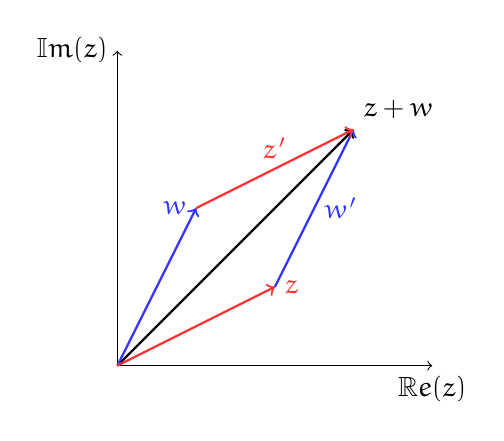
\begin{tikzpicture}
\draw [ <->] (0,4) node[left]{$ \ib $} -- (0,0) -- (4,0) node[below]{$ \rb $};
\draw [thick,->] (0,0) -- (3,3) node[above right]{$ z + w $};
\draw [blue!80,thick,->] (0,0) -- (1,2) node[left]{$ w $};
\draw [red!80,thick,->] (0,0) --(2,1) node[right]{$ z $};
\draw [blue!80,thick,->] (2,1) -- (3,3) node[right,midway]{$ w' $};
\draw [red!80,->,thick] (1,2) -- (3,3) node[above,midway]{$ z' $}; 
\end{tikzpicture}
\caption{Vector Addition}
\end{center}
\end{figure}
\end{document}